% !TeX spellcheck = it_IT
% TeX program = xelatex
\documentclass[aspectratio=169]{beamer}
\usepackage[italian]{babel}
\usepackage[utf8]{inputenc}
\usepackage[T1]{fontenc}


\newcommand{\mytitle}{Introduzione al profiling di applicazioni}

%\usepackage{libertine}
\usepackage{graphicx}
\usepackage{wrapfig}
\usepackage{tcolorbox}
\usepackage{tikz}
\usepackage{graphicx}
\usetikzlibrary{calc}

\usetheme[progressbar=foot]{metropolis}

\title{\mytitle}
\author{Ludovico Pavesi}
%\institute{Linux Day 2020}
\date{2020-10-24}

\definecolor{giallone}{HTML}{ffc928}
\definecolor{grigione}{HTML}{dbdbdb}
\setbeamercolor{alerted text}{fg=giallone}
\setbeamercolor{example text}{fg=grigione}
\setbeamercolor{progress bar}{fg=giallone}
\setbeamercolor{frametitle}{fg=black, bg=giallone}
\setbeamertemplate{footline}{\strut} % removes page numbering,

\begin{document}
	
	\frame{\titlepage}
		
	\begin{frame}
		\frametitle{Chi sono io}
		Un \textbf{umile programmatore} C++ e talvolta LISP in una grande azienda.
		
		Per qualche motivo scrivo anche codice PHP e Python e amministro server e tante altre belle cose per WEEE Open (\href{http://weeeopen.polito.it}{weeeopen.polito.it}).
	\end{frame}

	\begin{frame}
		\frametitle{Cos'è il profiling}
		Tecnica di \textbf{analisi} del software finalizzata all'\textbf{ottimizzazione}.
		
		Può riguardare:
		\begin{itemize}
			\item Tempo impiegato (da ogni istruzione, funzione, blocco di codice, etc...)
			\item Istruzioni eseguite (da ogni funzione, blocco di codice, etc...)
			\item Memoria occupata
			\item Cache hit/miss
		\end{itemize}
	\end{frame}

	\begin{frame}
		\frametitle{Cos'è il profiling}
		Tecnica di \textbf{analisi} del software finalizzata all'\textbf{ottimizzazione}.
		
		Può riguardare:
		\begin{itemize}
			\item Tempo impiegato (da ogni funzione, blocco di codice, etc...)
			\item Istruzioni eseguite (da ogni funzione, blocco di codice, etc...)
			\item Memoria occupata
		\end{itemize}
	\end{frame}

\begin{frame}
	\frametitle{Perché si fa}
	\textbf{Ottimizzazione}: meno istruzioni eseguite, meno tempo impiegato, meno memoria occupata, etc...
	
	Vantaggi per:
	\begin{itemize}
		\item Utenti: software più reattivo, requisiti di sistema più bassi
		\item Server: meno server necessari o meno potenti, ogni server può gestire più utenti
		\item Ambiente: di solito meno istruzioni eseguite, meno elettricità consumata
	\end{itemize}
\end{frame}

\begin{frame}
	\frametitle{Quando si fa}
	\textit{Premature optimization is the root of all evil} — Donald E. Knuth
\end{frame}

\begin{frame}
	\frametitle{Come si fa}
	Con un profiler.
	
	Quale utilizzare \textbf{dipende} dal linguaggio, integrazione con IDE e altri strumenti, etc...
	
	Vedremo:
	
	\begin{itemize}
		\item Profiler di tempo/istruzioni: Callgrind, VisualVM
		\item Visualizzatori: KCacheGrind, Qt Creator, VisualVM
	\end{itemize}
\end{frame}

\begin{frame}
	\frametitle{Concetti generali}
	Due tipi di profiler:
	\begin{itemize}
		\item \textbf{Sampling}: misure a campione ogni tot
		\item \textbf{Instrumented}: dati precisi forniti da VM, interprete, debugger, software stesso, ...
	\end{itemize}

	\begin{table}[htbp]
		\def\arraystretch{1.8}%
		\begin{tabular}{l l l}
			             & Precisione & Velocità \\ \hline
			Sampling     & Bassa      & Alta     \\ \hline
			Instrumented & Alta       & Bassa    \\ \hline
		\end{tabular}
	\end{table}
\end{frame}

\begin{frame}
	\frametitle{Sampling}
	\centering
	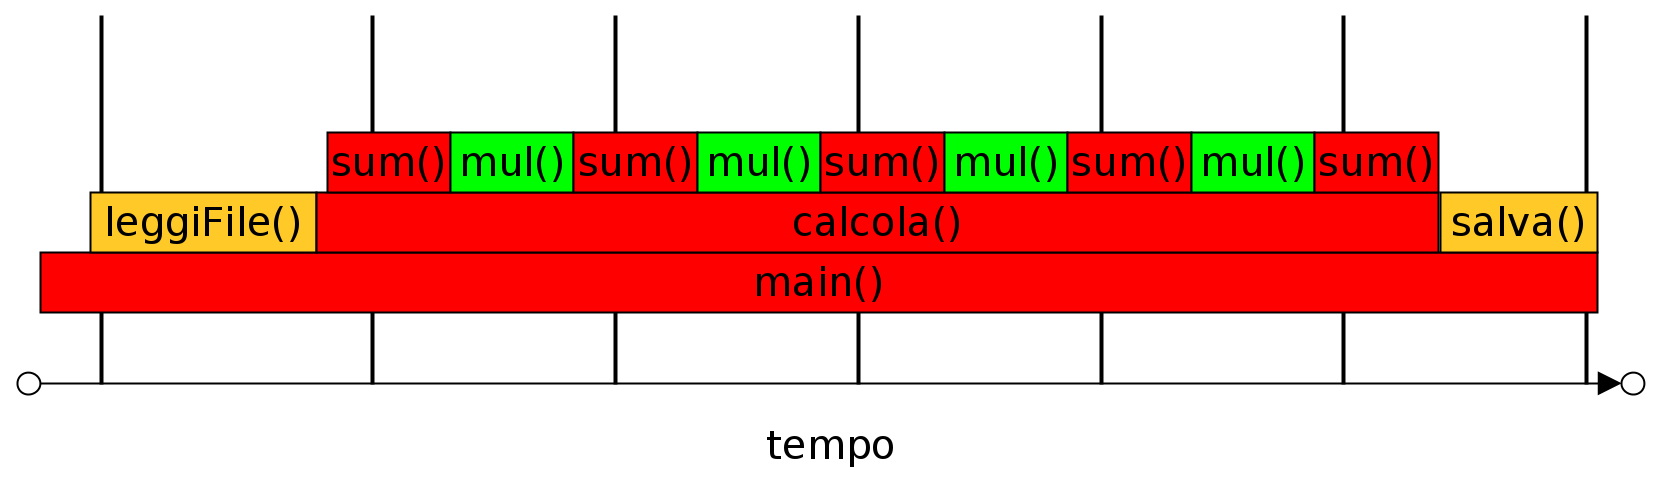
\includegraphics[width=\linewidth]{sampling}
\end{frame}

\begin{frame}
\frametitle{Instrumented}
\centering
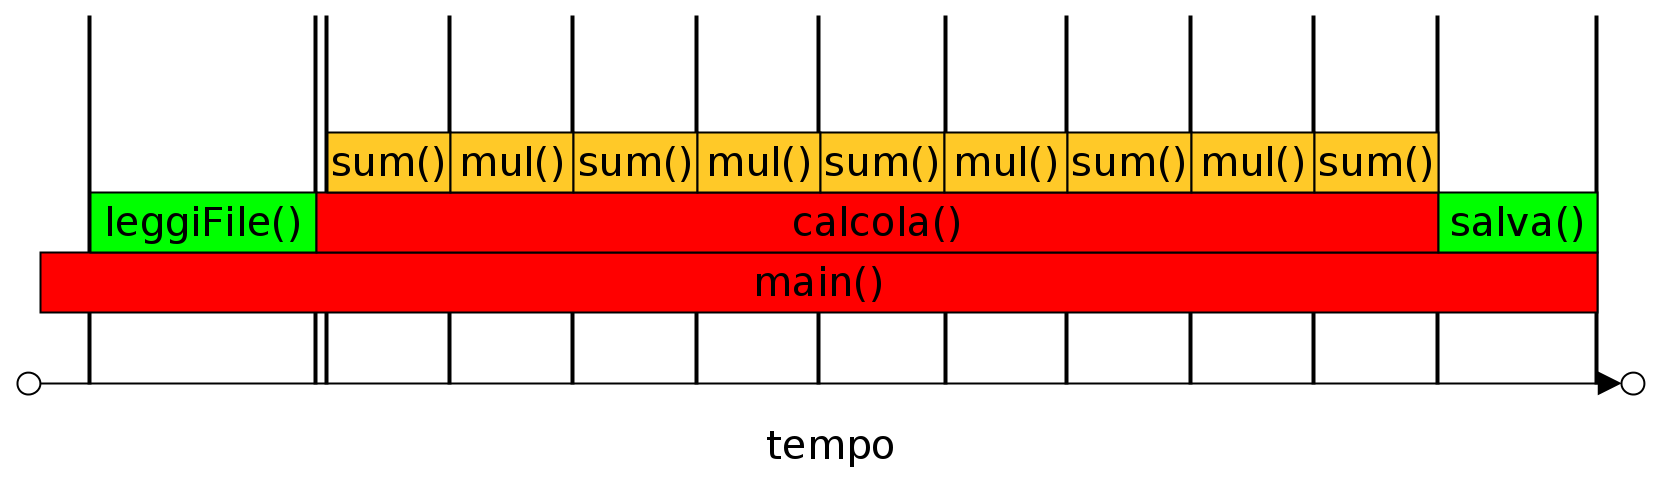
\includegraphics[width=\linewidth]{instrumented}
\end{frame}


\begin{frame}
	\Huge\centering Passiamo al codice!
\end{frame}

	\begin{frame}
		\frametitle{Fine}
		%{\centering\Huge Fine\par}
		{\centering\Huge Grazie per l'attenzione\par}
		{\centering\large Domande?\par}
		
		\vspace{5em}
		Codice sorgente: \href{https://github.com/lvps/talk-profiler}{github.com/lvps/talk-profiler-linuxday-2020}
	\end{frame}
	
\end{document}